\section{Background}
\subsection{A Preface On Humanity And The Climate}
\begin{flushleft}\emph{
The development of humanity is not unlike the chirography of an Aristotelian tragedy. It starts with a simple/primitive species cradling a noble cause - to improve their chances of survival. Here the protagonist (humankind) develops a fatal flaw: insecurity and latent destruction of their home due to a sudden rise to power.
Having acknowledged this flaw, we now strive to improve our understanding of the universe, correct past mistakes and stem the tide of inevitable change. \vspace{\baselineskip}\linebreak
With tragedy being an imitation not of humanity, but of action and life, happiness and misery, it is only expected that such a comparison to our current affairs should stir feelings of catharsis when exploring our need for research and scientific advancement.
It is with that I begin this thesis with the beginning of the planet, its atmosphere and consequently the start of humankind.
}
\end{flushleft}


\subsection{Formation Of The Atmosphere}
 ~4.5 billion years ago the Earth began as a disk of dust and gas orbiting our sun. The movement of such gasses produces a resonant drag instability, which causes them to clump together \citep{drag,planet}. As these `clumps' become denser, other forces come in to play and further increase their size. These eventually produced the hot mix of gas and solid, which was to become Earth.
 As the Earth cooled, the volatile components of the primordial gas cloud surrounding it begins to form an atmosphere. %Volcanic eruptions (outgassing) from the Earth's surface
At this point, oxygen was not only absent in the atmosphere but also had many sinks within the Earths anoxidised crust. It was not until oxygenic photosynthesis (\citep{oxygenicphotosynthesis}) that the concentrations of oxygen in the atmosphere started to increase. Eventually the development of multicellular cyanobacteria\footnote{The phylum of photosynthetic prokaryotic (cells not containing a distinct nucleus) bacteria - e.g. blue-green algae} resulted in biologically induced oxygen accumulating in the atmosphere, \citep{multicellular}. This led to the most significant climate event in the history of the planet: the Great Oxygenation Event (2.5 billion years ago), \citep{oxidation}. This increase in oxygen allowed organisms to become larger and more active, eventually resulting in the human race.


\subsection{Rise Of The Homo Sapiens (`Wise Man')}
2-6 million years ago there were many varieties of the `homo' genus (\autoref{fig:skulls},\cite{skull}). ~70,000 years ago homo sapiens came into existence and started the cognitive revolution. Here again in brain size increased communication, tool development and analysis capabilities. However, the evolutionary brain enlargement required an increase in net energy intake \citep{brainenergy} (the brain makes up for 2-3\% of human body mass but consumes 25\% of the body's energy at rest \citep{sapiens}).

A change of diet \citep{diet} soon addressed this energy imbalance, provisioning and sharing (cooperative breeding) and tool-assisted processing such as cooking \citep{cooking} - the first known case of anthropogenic indoor air pollution. The increase of cerebral power eventually led to the agricultural revolution\footnote{Domestication of plants and animals.} (12,000 years ago) and the scientific revolution\footnote{ humankind admits ignorance and gain unprecedented control} (500 years ago), \citep{sapiens}.

 Air pollution and climate have always been a concern for the human race. Such disquietude was first documented 6000 years ago with the ancient greeks  (lead in the air) \citep{skeptical} and the Romans (Rome was reported to have a `stink of soot and heavy air') \citep{roman}. In 1285 the smell of burning jet\footnote{The lowest rank of coal and very common at the time.} drove the Queen of England to leave Nottingham and 22 years later King Edward released the first air pollution act \citep{coal1}. In the 18th century the United Kingdom entered the Industrial age, here combustion was used to power machines and replace hand tools with mechanical ones. With this started the age of technology and automation - a process requiring energy, and thus increasing emissions to the atmosphere. In the present day technology is ever increasing in efficiency - however the rate of this is not yet suficient to mitigate any damage already caused.


\section{Motivation (How The Atmosphere Affects Us)}
The atmosphere constitutes an integral part of the Earth system. It is responsible for shielding the planatary surface from harmful radiation; allowing the transport of energy (weather and climate forcing), and interacting with the biosphere. This section explores the many roles of the atmosphere, and consequently, the interests and motivation of climate and atmospheric science. We start with the composition of the atmosphere and air quality (\autoref{sec:airq}), and then relate this to the different roles of ozone (\autoref{sec:ozonerole}), concluding on changing climate and radiative forcing, for with OH plays a vital role (\autoref{sec:climatechange}).



\subsection{Air Quality - It Is The Air We Breathe}\label{sec:airq}
The atmosphere consists mainly of nitrogen (\ch{N2}) and oxygen (\ch{O2})\footnote{These form  99\% of its dry-air total mass}, in addition to a vast range of other species \citep{ac}. Human beings rely on oxygen to convert sugars and fatty acids into energy. The procurement of this lies through the breathing of the air surrounding us - the composition of which can have dire effects on our respiration system. Pollutants such as particulate matter (PM), ozone (\ch{O3}), nitrogen dioxide (\ch{NO2}) and sulphur (\ch{SO2}) dioxide can cause respiratory problems, heart disease, strokes, cancer and chronic obstructive pulmonary disease \cite{who}. Over 80\% of people who live in urban environmets\footnote{Which measure the levels of air pollution.} are exposed to poor air quality levels exceeding the recommended limits by World Health Organisation, air quality poses a significant risk to human life - It is estimated that 4.2 million premature deaths globally are linked to ambient air pollution\footnote{A similar number can also be attributed to indoor air pollution - which also falls under the umbrella term of Air-Quality.} (\autoref{fig:who}).

\begin{figure}[H]
  \centering
  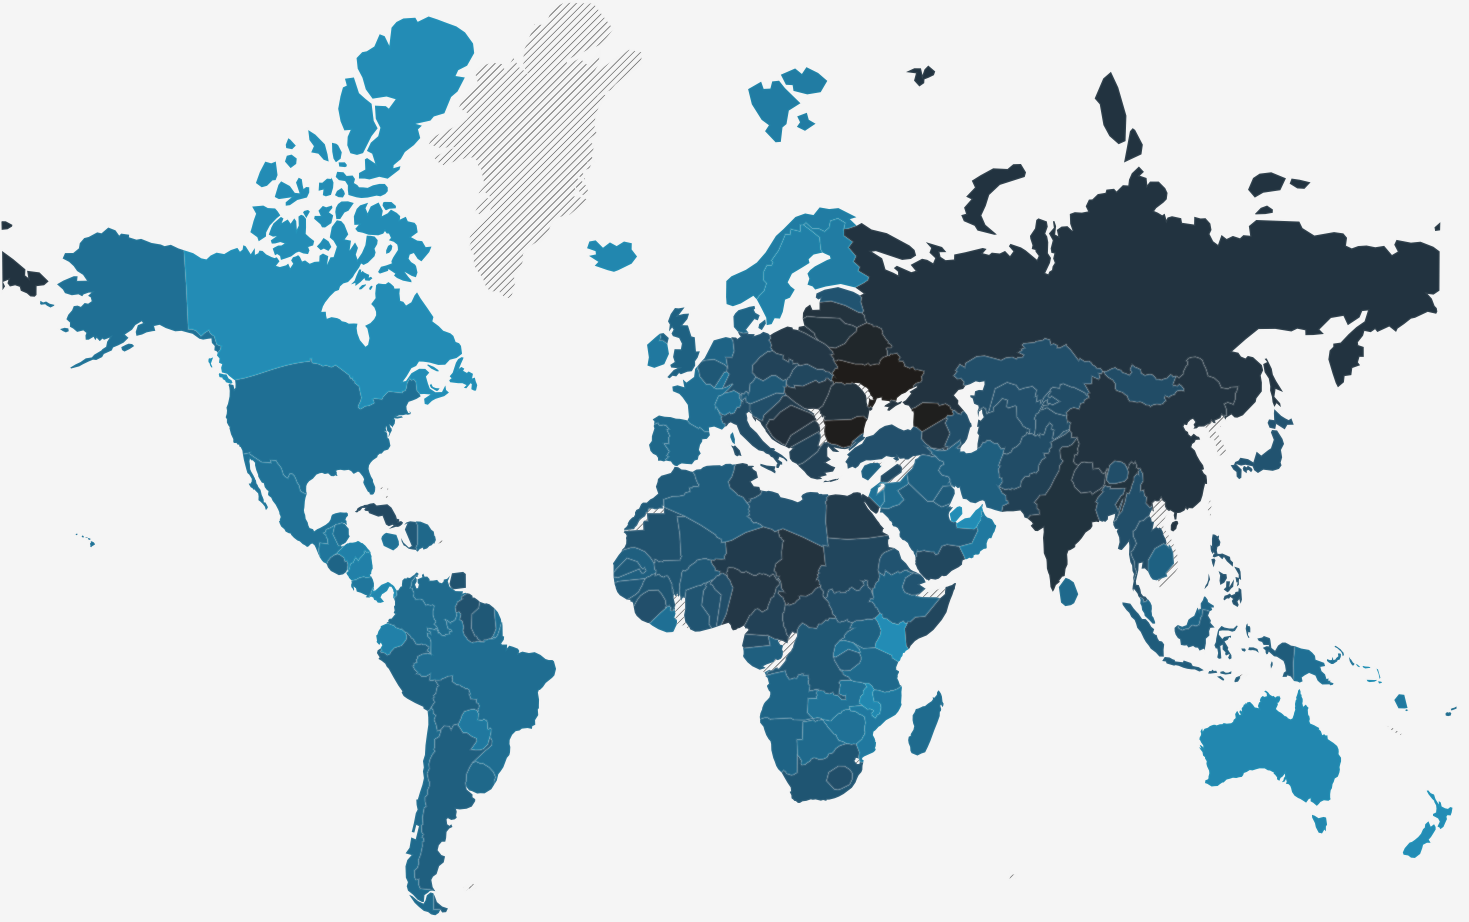
\includegraphics[width=\textwidth]{who.png}
  \caption{\textbf{Reported deaths attributed to air pollution by country (2016)}A cartogram (and cloropleth) showing the number of premature deaths attributed to ambient air pollution per 100,000. The colour bar range is from 9 in Canada (light blue) to 170 in eastern Europe (navy) people.  Data Source:\citep{whodata}}
  \label{fig:who}
\end{figure}
%
\subsection{Stratospheric Ozone - The Protective Barrier}\label{sec:ozonerole}
Ozone plays a vital role in the stratosphere. This was seen in the 1980s where the use of Cloro Fluro Carbon (CFC) aerosols resulted in the thinning of the atmospheric ozone \citep{ozonehole}\footnote{Here the chlorine attacks the double bond and `steals' an oxygen atom from the \ch{O3} molecule.}. This resulted in an increase in UV-B radiation, and in consequence skin cancers, immune suppression and disorders of the eye \citep{o3damage}. Due to this, the Montreal Protocol on Substances that Deplete the Ozone Layer was put into place to reduce the adverse effects experienced by humans and the Earths surface \citep{montreal}. As part of this, CFCs are still being phased out resulting in a gradual decrease in the damage of the ozone hole.


\subsection{Changing Climate} \label{sec:climatechange}
Over the last 30 years, a large body of scientists has established that humans have a warming effect on the planet \citep{IPCC1990Science,IPCC1995Science,IPCC2007Science,IPCC2013Science,ipbes}. Here it has been shown that changes in temperature can lead to the melting of glaciers, rise of sea levels, extreme weather events and the extinction of many species.

The impact of this resulted in the nations of the world to develop a `legally binding' agreement to combat climate change (the Paris agreement) \citep{paris1,paris}. However, a recent analysis on the current state of the world outlines that the failure to set, implement and without adequate targets and procedures within the last decade mean that we now need to do `four times the work, or [do it in] one-third of the time' \citep{failparis}.



\section{Tropospheric Chemistry}

The lowest part of the atmosphere (<18km)\footnote{18km at the tropics, 17km in the mid-latitudes and 6km at the poles. } is called the troposphere. This contains ~75\% of the mass of the atmosphere, and comes from the greek $\tau\rho o \pi o \varsigma$ which means `way' or `turn towards change'. This describes the turbulent mixing that happens due to friction in the lower 2km of the atmosphere (the boundary layer). As the troposphere is the closest part of the ground, this where most of the complex chemistry which affects us at the surface happens. This section describes the underlying chemical processes which exist in the atmosphere.




\subsection{Ozone Production/Loss}\label{sec:o3prod}
In the troposphere, the mixing ratio of ozone is controlled by the photostationary state relationship (\autoref{eqn:o1}-\ref{eqn:o3}).
Since the concentrations of ozone (20-60 pp\textbf{b}v)\footnote{ppbv: parts per billion volume} are often much higher than that of the nitrogen oxides, NO (1-60 pp\textbf{t}v)\footnote{pptv: parts per trillion volume} and \ce{NO2} (5-70 pp\textbf{t}v), the rapid rate of reaction between \autoref{eqn:o1} does lead to a net change in \ch{o3} concentration \footnote{In urban areas NO concentrations may rise to be be greater than those of \ce{O3} during the night. This leads to a decrease in from \autoref{eqn:o1}} \citep{fundamentals}.



\begin{equation}
  \centering
\ce{NO + O3 ->[k1] NO2 +O2} \label{eqn:o1}
\end{equation}
\begin{equation}
  \centering
 \ce{NO2 ->[hv (J)] NO + O }\ \ \ (\lambda < 420nm) \label{eqn:o2}
\end{equation}
 \begin{equation}
   \centering
\ce{O + O2 + M ->[k2] O3 + M}\label{eqn:o3}
\end{equation}

Using \autoref{eqn:o1} and \autoref{eqn:o2} it is possible to describe the change in \ce{NO2} as:

\begin{equation}
  \frac{d[NO_2]}{dt} = k1[NO][O_3] - J[NO_2]
  \label{eqn:ono2}
\end{equation}

If the relative change of \ce{NO2} is small, it can be thought of as being in a steady-state. This means that \autoref{eqn:ono2} can be simplified to produced a relationship between \ch{O3, NO} and \ch{no2} in steady-state (\autoref{eqn:oo3}). Here if any two concentrations are known, the third can be calculated.

\begin{equation}
  [O_3] = \frac{J[NO_2]}{k1[NO]}
  \label{eqn:oo3}
\end{equation}

As ozone is a secondary pollutant (made not emitted), and its primary reaction produces a null cycle, the production of ozone in the atmosphere requires an increase in nitrogen dioxide livnconcentraions.

\subsection{The Nox Cycle}\label{sec:noxcycle}
Ozone production/loss in the troposphere is directly dependant on the concentration of available Nitrogen Oxides (NOx) (\autoref{sec:o3prod}). These are predominantly emitted by motor vehicles and power stations and can are known to cause respiratory problems in children and asthmatics as well as disrupting terrestrial and aquatic ecosystems \citep{eea}. Although NOx may be released naturally, the anthropogenic influence on their emissions was highlighted in early 2020 where the COVID-19 coronavirus disrupted travel across mainland china, causing a significant drop in anthropogenic emissions - \autoref{fig:chinanox}.

\begin{figure}[H]
    \centering
    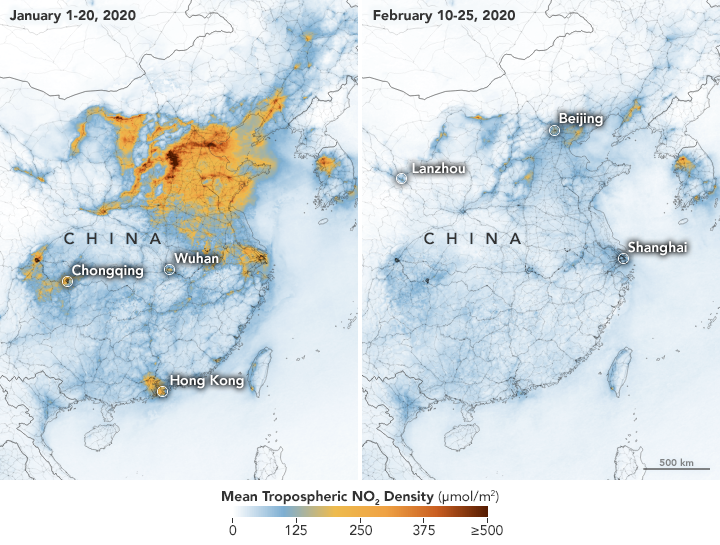
\includegraphics[width=0.7\textwidth]{china_trop_2020056.png}
    \caption{\textbf{Changes in NOx concentrations due to anthropogenic emissions.} A reduction in activity and trasport resutls in a large decrease of Nitrogen dioxide concentrations in the troposphere. Source: \citep{chinanox}}
    \label{fig:chinanox}
\end{figure}

During the day nitrate (\ce{NO3}) radicals can be formed through the reaction with \ch{O3}: \autoref{eqn:ono2} and \autoref{eqn:nno2}, however this is quickly destroyed through rapid photolysis (\autoref{eqn:nno3}) \citep{nitrate}. Photolysis reactions such as \autoref{eqn:nno3} and \autoref{eqn:o2} are no longer possible and th ozone production process shuts down.

\begin{equation}
  \ce{NO2 + O3 ->[k3] NO3 + O2}
  \label{eqn:nno2}
\end{equation}

\begin{equation}
  \ce{NO3 ->[hv] NO2 + O(3P)}
  \label{eqn:nno3}
\end{equation}


 The increased amount of \ce{NO3} can now react with \ce{NO2} to produce dinitric pentoxide (\ce{N2O5}) and an aqueous nitric acid (\ce{HNO3}) - \autoref{eqn:n2o5} and \autoref{eqn:hno3}. \autoref{eqn:n2o5} is a three-body forwards pressure dependant reaction and a reverse temperature dependant reaction. During the day at the lower troposphere, it is warm, and this can occur within seconds, however, at night or high altitudes it can take anywhere from hours to months \citep{fundamentals}.


\begin{equation}
  \ce{NO3 + NO2 <=>[M] N2O5 + O}
  \label{eqn:n2o5}
\end{equation}

\begin{equation}
  \ce{N2O5 + H2O ->[k4] 2HNO3}
  \label{eqn:hno3}
\end{equation}



\subsection{Hox Cycle}
The hydroxyl (OH) radical is central to tropospheric chemistry and a major sink for many of the greenhouse gasses (including ozone) \citep{olson}. Its primary source of production is through the action of UV in sunlight to photolyse ozone \citep{fundamentals}:


\begin{equation}
  \ce{O3 ->[hv] O1D}
\end{equation}

\begin{equation}
  \ce{O1D + H2O -> 2OH}
\end{equation}

As OH is highly reactive ($<1$ seconds - \autoref{fig:timescales}) it is not transported a long distance and only exists during daytime (when it is still being produced). In reacting with a VOC, the hydroxyl radical scavenges hydrogen to form a radical species and water (\ch{h2o}). This produced radical species can then move on to react with \ch{O2} to produce a \ch{RO2} species (\autoref{fig:hox}). Additionally, reaction with OH can lead to the catalytic destruction of \ch{o3}. This provides the hydroperoxide radical (\ch{HO2}).

\begin{equation}
  \ce{OH + O3 -> HO2 + O2}
\end{equation}

Unlike OH, \ch{HO2} can exist both during daytime and night. It can further react with ozone to reproduce the hydroxyl radical and create two \ch{o2} molecules:

\begin{equation}
  \ce{HO2 + O3 -> OH + O2 + O2}
\end{equation}

Its loss depends on the NO mixing ratio, where if NO $>10$ pptv, \ch{HO2} will react predominantly with the NOx species. At lower concentrations (3-10 pptv) \ch{HO2} reacts mainly with ozone, and at deficient concentrations, it reacts mostly with itself \citep{finlayson}. Combined OH and \ch{ho2} form the HOx species, and the cycle in \autoref{fig:hox}.

\begin{figure}[H]
  \centering
  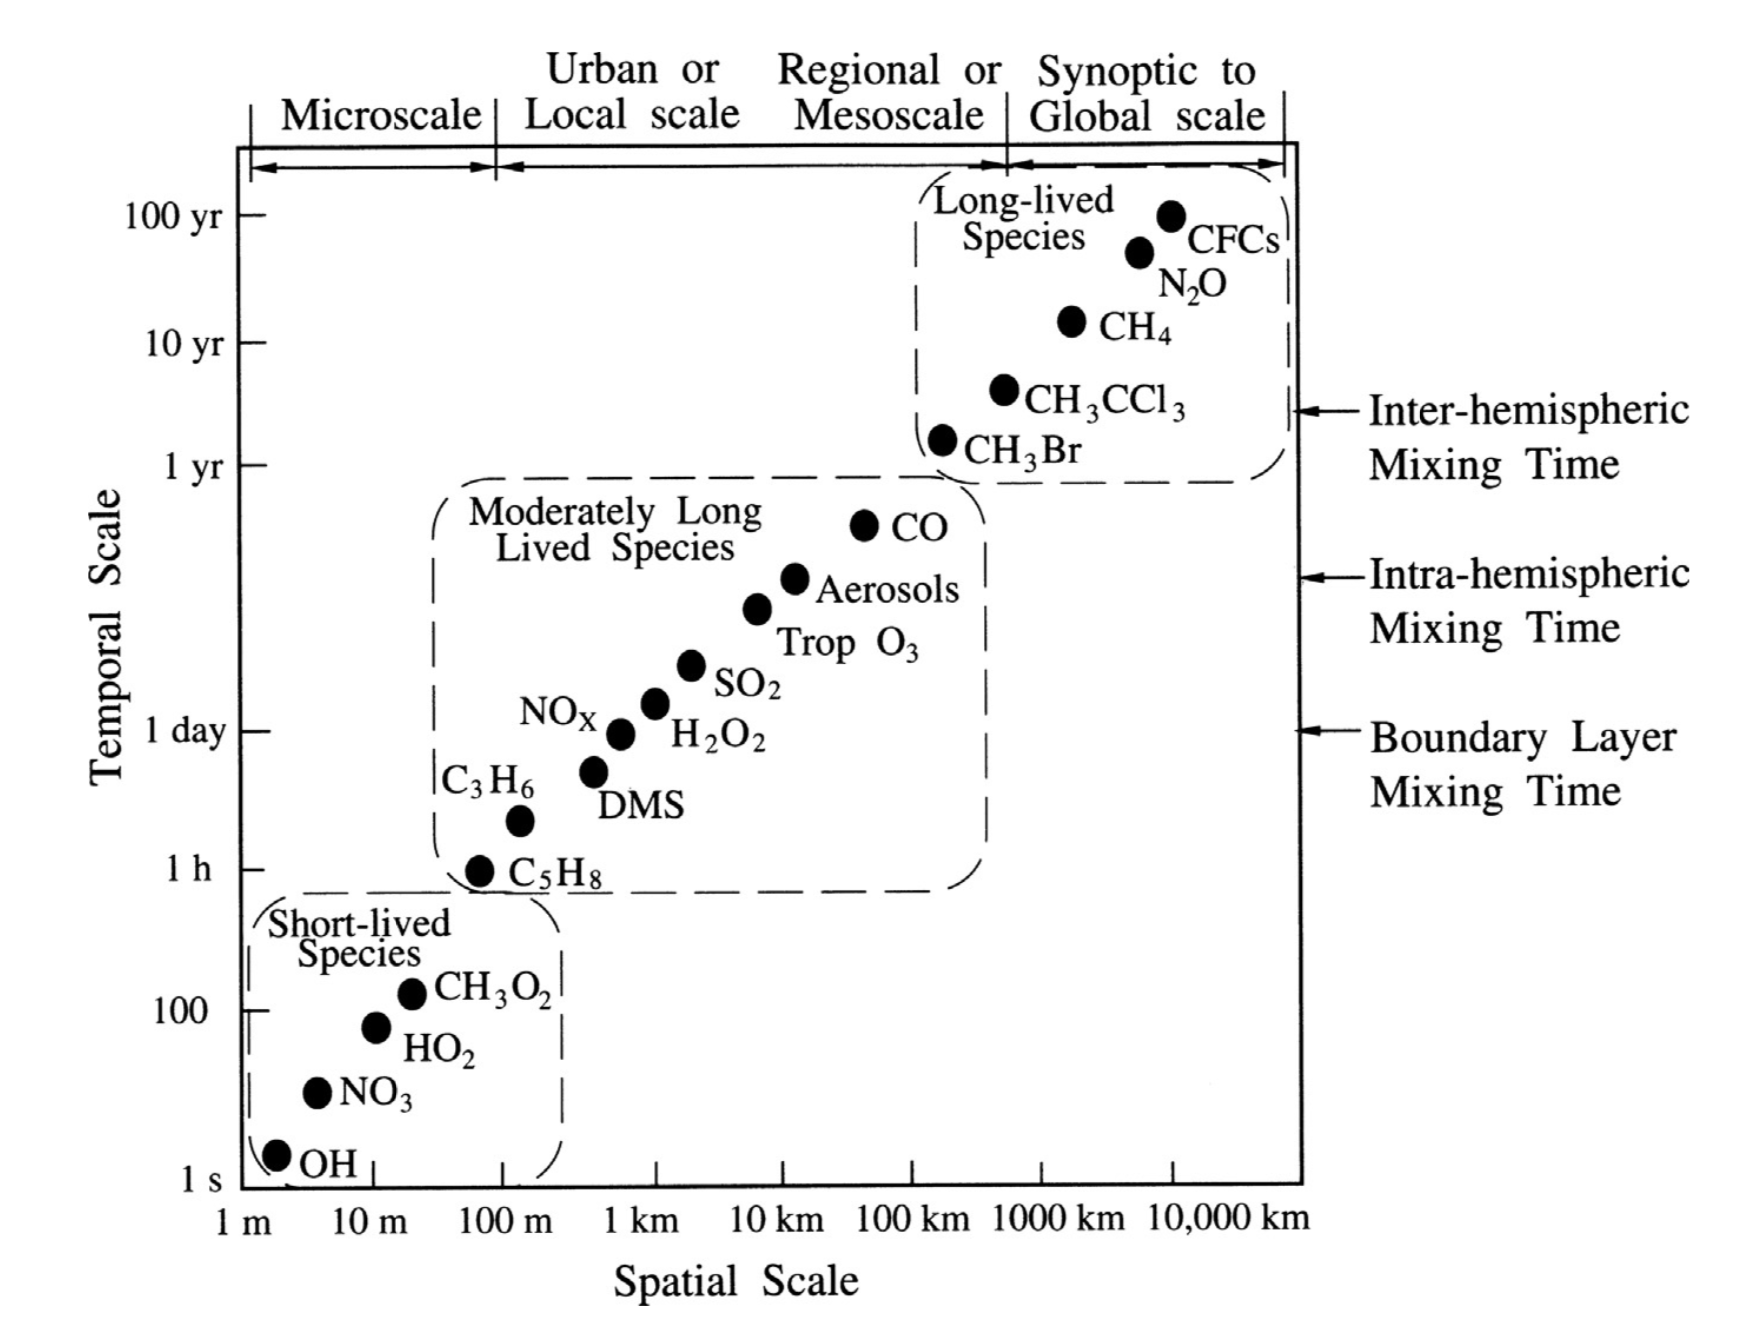
\includegraphics[width=0.7\textwidth]{timescales.png}
  \caption{\textbf{Spatial and temporal scales of variability of atmospheric species.} This shows that the longer lived a species, the further it is likely transported through the atmosphere. Source: \citep{transporttime}}
  \label{fig:timescales}
\end{figure}

\begin{figure}[H]
    \centering
    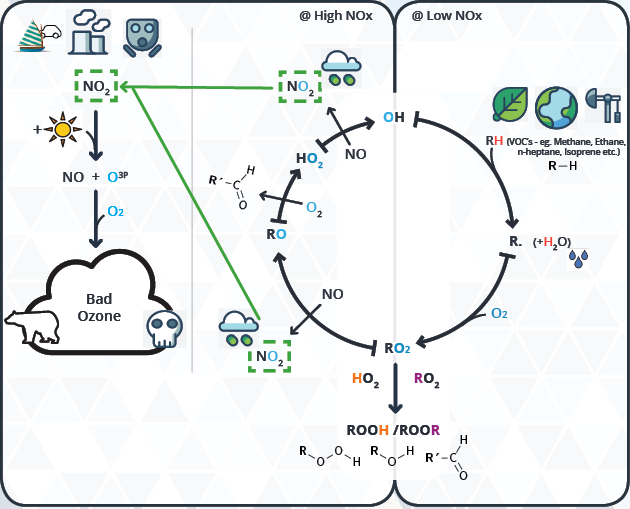
\includegraphics[width=0.7\textwidth]{hoxcycle.png}
    \caption{\textbf{The HOx cycle.} The OH aids in the oxidation of VOCs, which makes them more water soluble - this allowing for their removal from the atmosphere. In a high NOx evironment the \ch{RO2} radicals can then reacti with NO to produce \ch{NO2}, and consequenty more ozone.}
    \label{fig:hox}
\end{figure}

\section{Modelling The Earth}
In the previous section, the air quality and its detrimental effects on human health were seen to influence policy for cities and industry.
For a policy to be passed there needs to not only evidence of the problem but a strong suggestion that any proposed changes will have the desired effect. As it is not possible to perform experiments on complex, and often unknown, chemistry at every location on the planet, we are forced to rely on the numerical simulation of the Earth System, and the constituent parts within it.
\subsection{Earth System Models (ESM)}
  ESMs are models capable of predict past or future interactions of the planetary system. They represent our foremost understanding of the complex interplay between land-surface (geosphere), ocean (hydrosphere), ice (cryosphere) and the air (atmosphere), and act as a surrogate to manual experimentation -  which is just not possible on the global scale.
ESMs can be split into individual parts. One example of this is the Chemistry section of the Goddard Earth Observing System (an integrated ESM and data assimilation model hosted by NASA's Goddard space flight centre \citep{geosgit}) - GEOS Chem. GEOS-Chem is a global 3D model of atmospheric chemistry which is driven by the meteorology provided by NASA \citep{geos}. Here the Earth is split up into cubic cells longitudinally, latitudinally, and vertically (\autoref{fig:gcm})\footnote{This image is not from GEOS-Chem.}. Each one of these cells performs several perturbations of the chemistry within them before any long-lived species are transported, and the process is repeated. If extracted separately, a single one of these cells may be used to explore the sensitivity of different species for a range of input conditions. This is the bases of the atmospheric box model.
\begin{figure}
  \centering
  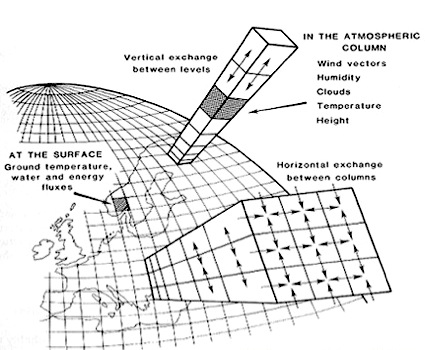
\includegraphics[width=0.6\textwidth]{gcm.jpg}
  \caption{\textbf{A diagram showing the longitudinal, lateral and vertical decomposition of a 3D global model.} (Diagram not of GeosChem.) Source: \citep{gcm}}
  \label{fig:gcm}
\end{figure}
\section{The 0D Chemical Box Model}
In exploring the sensitivities of individual species within a simulation, it is possible to use a zero-dimensional box model. This is, in essence, a single cell within the global structure which has been constrained in location and height (pressure). A box model allows for better in-depth analysis of the chemistry within a model, without any of the overhead of having to run it for the entire planet. Such studies make zero-dimensional models perfectly suited for studying the sensitivity of chemical schemes under a range of conditions, for example, \citep{dsmacc}.

In general, a box model consists of two main parts - a mathematical representation of the reactions in the atmosphere and the rate they occur (this is known as a mechanism); and a method to propagate this chemistry forwards in time (the integrator).



\subsection{Chemical Mechanisms}
Mechanisms are at the heart of every chemistry simulation. They are a mathematical representation of the possible reactions ( and the rates at which these may occur ) which describe the evolution of the atmosphere within a numerical model. Different models contain varying levels of chemical complexity depending on their individual foci. However, there is a need for a `gold standard' or `benchmark mechanism' which contains a comprehensive representation of the current `state of the science'. For the last decade, the benchmarking mechanism for both the UK and internationally has been the Master Chemical Mechanism \citep{mcm} (this shall be described throughout the rest of this thesis).


\subsection{Numerical Integration}
Using a mechanim it is possible to determine how quickly each species in a reaction is changing at a certain set of conditions using its a slope or derivative. In this way, integration allows us to find the change in concentration over time as well as the rate at which this is happening.  Taking the reaction of \ch{N2O5} (\autoref{eqn:numerical1}), we can write the rate of change for each species over time (\autoref{eqn:numerical2})\footnote{This is also known as the flux.}. In integrating this equation, we are able to calculate the actual change in concentration (\autoref{eqn:numerical3}) - this is the foundation of atmospheric models.
\begin{equation}
\ce{N2O5 ->    NO2} + \ce{NO3}
\label{eqn:numerical1}
\end{equation}
\begin{equation}
\ce{ d[N2O5]/dt ->    d[NO2]/dt} + \ce{d[NO3]/dt}
\label{eqn:numerical2}
\end{equation}
\begin{equation}
\ce{ \int d[N2O5]/dt ->    \int d[NO2]/dt} + \ce{\int d[NO3]/dt}
\label{eqn:numerical3}
\end{equation}
\subsubsection{Non-Stiff Equations}
Non-stiff ordinary differential equations are made up components which all evolve at similar timescales. They can easuly be solved by explicit (calculate the next step using the current time only) numerical methods which can be solved with the forward Euler\footnote{\textbf{Euler:}Evaluate gradient at the time point, move forward in time and repeat.}, Runge Kutta \footnote{\textbf{RK4:}The next value is determined by the present value combigned with the weighted avarage of 4 increments across an interval $h$.} or Verlet methods\footnote{\textbf{Verlet:}A central difference method to find the gradient using the avarage of a forwards and backwards timestep.} \citep{advnummeth,wild}.
\subsubsection{Numerically Stiff Equations (Atmospheric Chemistry)}
Unfortunately, chemical lifetimes within the atmosphere range several orders of magnitude (\autoref{fig:timescales}). This creates a numerically stiff system that requires the step size to be chosen based on the most rapid component, which can lead to inefficiency in the computation of the entire system. Solvers for stiff equations usually create and evaluate the Jacobian matrix (a matrix of second-order partial derivatives describing the effect species have on each other).

Standard solvers include Backward Differentiation Formulas (known as the `gear' method and implemented as the LSODE solver in \citep{kpp}),  implicit Runge Kutta and the Rosenbrock methods. Gear methods are multistep methods with high stability and have been applied to a range of atmospheric chemistry models \citep{gear, geos, fundamentals}.
The Rosenbrock method can be likened to a linearly-implicit Runge Kutta method which uses the Jacobian matrix directly within the integration formula (solved at each stage) to avoid solving for a non-linear system \citep{solvers}. This provides an efficient solver with modest accuracy (less than $10^{-5}$) which is more than suitable for use within atmospheric chemistry calculations \citep{solvers,rosenbrock}.


\subsection{The Model Development Cycle}
Scientific understanding is the product of many cycles of trial and error, \autoref{fig:devcycle}. In atmospheric chemistry, we start with a hypothesis or a question, e.g. will change X has a negative response on Y. We then construct a theoretical model to represent the chemistry within. This chemistry is updated to reflect the rates and reactions that have been recorded in laboratory/chamber experiments. This cycle is then repeated until the model, and real-world observations produce a comparable result.
It is essential to point out that improving the predictive capabilities of a model are iterative tasks which both feedback and respond to changes in our understanding of atmospheric reactions.



\begin{figure}[H]
    \centering
    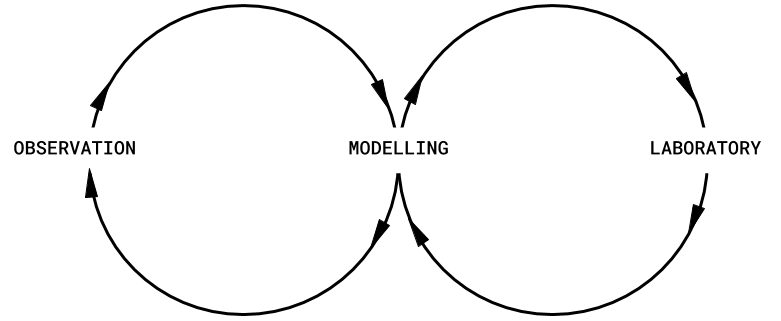
\includegraphics[width=0.6\textwidth]{devcycle.png}
    \caption{\textbf{The scientific development cycle.}This shows the iterative nature between modelling, observation and laboratory experimentation}
    \label{fig:devcycle}
\end{figure}

 \subsection{The Dynamically Simple Model Of Atmospheric Chemical Complexity}

Within this thesis, the Dynamically Simple Model of Atmospheric Chemical Complexity (DSMACC) was used to run model simulations. This a simple box model designed for the comparison of a range of gas-phase chemical schemes under different conditions \citep{dsmacc}.
 The DSMACC model uses the Kinetic PreProcessor (KPP) to convert a chemical mechanism into the set of ordinary differential equations which can be solved using a suite of FORTRAN numerical integrators it provides \citep{kpp}. The Tropospheric and Ultraviolet (TUV) model from \cite{tuv} is used to calculate the strengths of different photolysis reactions for the mechanism. These are determined at the start of a simulation and then predicted using cubic splines \citep{dsmaccgit}. This is the model setup that will be used to propagate the chemistry forwards in time using the Rosebrock integrator.

\section{Thesis Layout}
This thesis will explore a series of methods for describing and understanding the complex chemistry which may exist as part of an atmospheric chemistry mechanism. The mechanism used is a near-explicit representation of our foremost understanding of how gas-phase chemistry in the troposphere reacts - the Master Chemical Mechanism, \citep{mcm}.
We begin by exploring the use of visualisation to convey complex scientific data (\autoref{ch1}). Next, we apply this to the representation of species in a mechanism and the relationships between them. It is found that the node-link style graph format is the most beneficial, the use of which is then explored further (\autoref{ch2}).
However, in doing so, sizeable complex networks are shown to reach the limits of human cognition and visual representation. A series of mathematic metrics are used to leverage our understanding of the species in a chemical network using graph theory (\autoref{ch3}). The use of computation to aid in graph analysis is further extended when graph clustering methods are applied as a method to similar group species within a chemical network (\autoref{ch4}). Finally in a bid towards the use of neural graph networks (see future work, \autoref{sec:futurework}), a range of different chemical representations for machine learning are explored using several dimensionality reduction algorithms (\autoref{ch5}).
